%%%%%%%%%%%%%%%%%%%%%%%%%%%%%%%%
\section{Overview}
\label{sec:detectors-fd-alt-ov}

This chapter describes an alternative far detector design for
DUNE. The first detector module to be installed will use the reference
design described in Chapter~\ref{ch:detectors-fd-ref}, however this alternative
 design is under consideration for one or more
subsequent modules. This design implements a dual-phase liquid argon
time projection chamber (LArTPC) augmented with a light-readout
system. ``Dual-phase'' refers to the extraction of ionization
electrons at the interface between liquid and gas argon and their
amplification and collection in the gas phase.

This dual-phase design is the result of 13 years of R\&D consisting of two
consecutive design study programs funded since 2008 by the European
Union: LAGUNA and LAGUNA-LBNO. The LAGUNA-LBNO design study was
concluded in August 2014.  In collaboration with industrial partners,
LAGUNA-LBNO designed an innovative, optimized and cost-effective
configuration for a long-baseline experiment.

The studies focused on the underground implementation of a very large
LAr detector (GLACIER) and produced many technical advances with respect to
the tank, field cage and cathode, charge multiplication, collection and readout, as well as 
advances in the areas of assembly sequencing and logistics for the detector and 
full costing. The full design and the related
technical developments are described in \anxlbnob, which was submitted to the
EU at the conclusion of the design study. This chapter describes the detector
configuration and components, and describes how the design meets the DUNE
far detector physics requirements.

The scope of a dual-phase far detector module for DUNE includes the design,
procurement, fabrication, testing, delivery, installation and
commissioning of the detector components:
\begin{itemize}
\item Charge-Readout Planes (CRP), including extraction grid, Large Electron Multiplier (LEM) and anode and readout planes
\item Cathode, field cage and high voltage system  
\item Electronics and data acquisition 
\item Chimneys, isolated volumes used for electronics feedthroughs 
\item Slow Controls
\item Light-readout system
\end{itemize}

The detector components and the liquid argon (LAr) will be housed in cryostats
provided by LBNF, described in \vollbnf.  Similar to the reference design, 
this alternative design satisfies the performance 
requirements on the DUNE far detector, described in Chapter~\ref{ch:detectors-fd-ref} for the reference design.
Parameters specific to the dual-phase design are listed in
Table~\ref{tab:FD_req}.

\begin{cdrtable}[Dual-phase (alternative) far detector performance parameters]{llll}{FD_req}{Performance parameters specific to the dual-phase far detector design}  
Parameter & Requirement & Achieved Elsewhere & Expected Performance \\ \toprowrule
Gas phase gain & 20 & 200 & 20-100  \\ \colhline
Electron Lifetime & 3~ms &  $>3$~ms 35-t prototype  & $>5$~ms \\ \colhline 
Minimal S/N after 12 m drift & 9:1 &  $>100$:1 & 12:1-60:1  \\ 
\end{cdrtable}

\subsection{Highlights of the Design}

This innovative dual-phase design is similar in many ways to the single-phase design,
but implements some unique features and offers several advantages over it, in particular:
\begin{itemize}
\item  higher gain, leading to a larger signal-to-noise ratio (S/N)
\item  larger fiducial volume, enabling very long drift paths
\item  lower detection threshold
\item  finer readout pitch 3~mm), implemented in two identical collection views, $x$ and $y$
\item  fewer readout channels (153600 vs 384000 for a reference design 10 kt module)
\item  the absence of dead material in the LAr volume
\end{itemize}

Following the GLACIER concept\cite{LAGUNA-LBNO-deliv} (see
Figure~\ref{fig:LBNO_50}), the DUNE dual-phase LArTPC detector design 
has a fully homogeneous liquid argon volume, in which electrons
drift upwards vertically towards an extraction grid just below the liquid-vapor interface. From there they
are extracted from the liquid into the gas phase, amplified, and
collected on a finely segmented
anode\cite{Badertscher:2013wm,Badertscher:2012dq,Badertscher:2010zg}. 
%
\begin{cdrfigure}[The \ktadj{50} LBNO detector, GLACIER]{LBNO_50}{The \ktadj{50} LBNO detector, GLACIER}
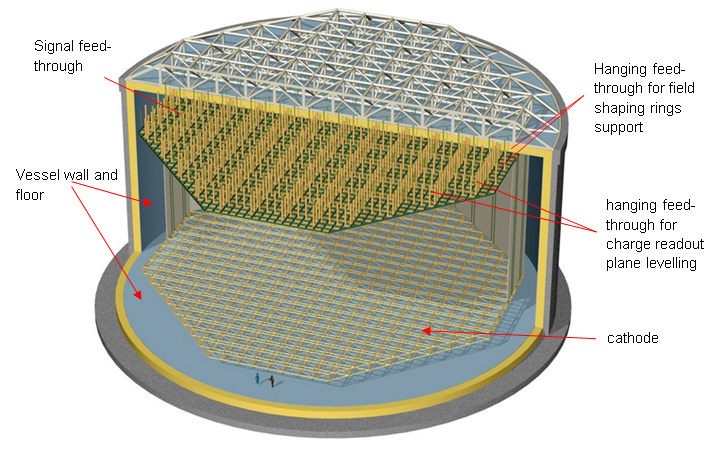
\includegraphics[width=0.9\linewidth]{LBNO50kton2}
\end{cdrfigure}
%

The electron amplification in the gas phase enables a robust and tunable signal-to-noise ratio. 
The detector configuration is similar to a single-phase LArTPC. The features of the dual-phase design, e.g., high gain, 
allow achieving very long drift paths and large detector dimensions while minimizing the number of readout channels.

\subsubsection{Charge Collection, Amplification and Readout}

An extraction efficiency of 100\% of the electrons from the liquid to
the gas phase is achieved with an electric field of the order of
2~kV/cm across the liquid-gas interface, applied between an 
extraction grid submersed in the liquid and charge amplification 
devices situated in the ultra-pure argon gas. 

These amplification devices, called Large Electron Multipliers (LEMs), are horizontally oriented 1~mm thick printed 
circuit boards with electrodes on the top and bottom surfaces. They are drilled
through with many holes that collectively form a micro-pattern structure;  
when a 3 kV potential difference is applied across the electrodes
the ionization electrons are amplified by avalanches (Townsend multiplication) occurring in the 
pure argon gas in this micro-pattern structure\cite{Bondar:2008yw} due to the high electric field (30 kV/cm).

The use of avalanches to amplify the charges in the gas phase increases
the S/N ratio by at least one order of magnitude with a typical gain of 20--100, significantly
improving the event reconstruction quality. It also lowers the
threshold for small energy depositions and provides a better
resolution per volumetric pixel (voxel) compared to a single-phase
LArTPC. 

The charge is collected in a finely segmented 2D ($x$ and $y$) readout anode
plane at the top of the gas volume and fed to the front-end electronics.   

The  collection, amplification and readout components are combined in an array of 
independent (layered) modules called Charge Readout Planes (CRPs), each of which is in
 turn composed of several 0.5$\times$0.5-m$^2$ units composed  by a LEM/anode sandwich. 
These units are embedded in a mechanically reinforced frame of FR-4 and Stainless Steel. The CRP structure integrates
as well the submersed extraction grid.which is is made by an array of X and Y oriented stainless steel wires, 0.1~mm in diameter with 3.125~mm
pitch. Thicknesses and possible biasing voltages for the different layers are indicated in Figure~\ref{fig:CRP_struct}.

\begin{cdrfigure}[Charge Readout Plane (CRP) structure]{CRP_struct}
{Thicknesses and HV values for electron extraction from liquid to gaseous Ar, their 
multiplication by LEMs and their collection on the $x$ and $y$ readout anode plane. The 
HV values are indicated for a drift field of 0.5~kV/cm in LAr.}
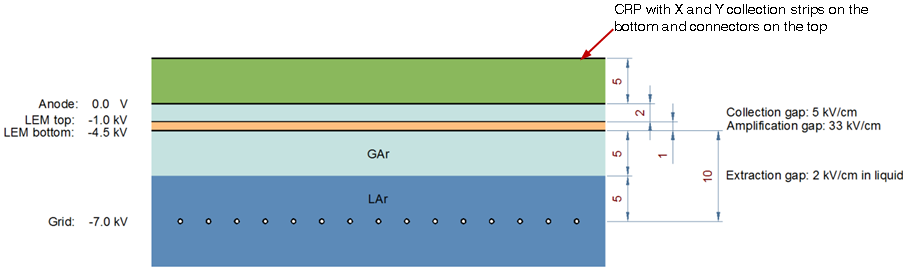
\includegraphics[width=\linewidth]{CRP_gaps.png}
\end{cdrfigure}

Each CRP  is independently suspended with stainless-steel ropes linked to the tank top deck. This suspension
system allows to adjust the CRP distance and parallelism with respect to the LAr surface and keep immersed the
extraction grid.

Figure~\ref{fig:CRP_unit1} shows the top of two side-by-side units and Figure~\ref{fig:CRP_unit2} shows the
$x$ and $y$ readout views

\begin{cdrfigure}[DUNE CRP 3~m$\times$3~m units.]{CRP_unit1} {Two DUNE CRP 3~m$\times$3~m units side by side. On the left one of the 79 equal 
CRP units, on the right the 1$^{st}$ CRP unit with a chamfered LEM/Anode Sandwich  for the insertion of the high voltage feedthrough.}
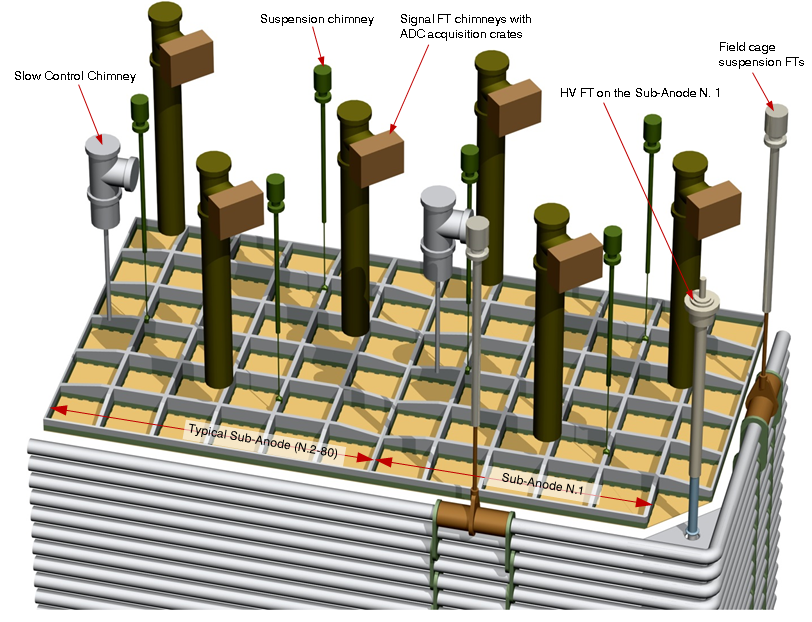
\includegraphics[width=.7\linewidth]{DUNE12_units}
\end{cdrfigure}
\begin{cdrfigure}[Signal collection in the X and Y views by the 3 SFT chimneys.]
{CRP_unit2}{Signal collection in the X and Y views of the  3$\times$3~m$^2$ DUNE CRP unit by the 3 SFT chimneys.}
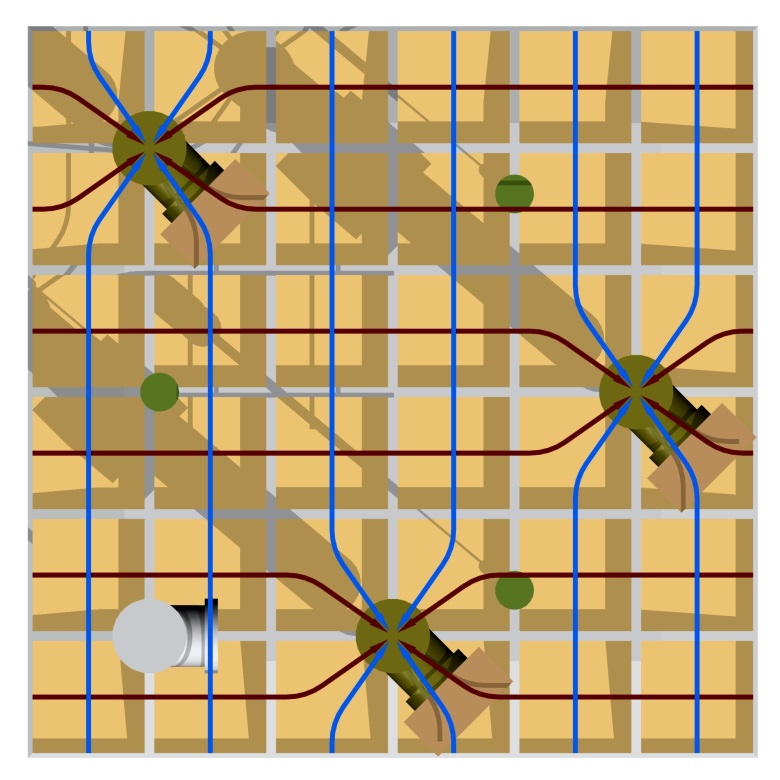
\includegraphics[width=.5\linewidth]{DUNE12_CRP}
\end{cdrfigure}

A CRP provides an adjustable charge gain (with a minimal required gain of 20) and two
independent, orthogonal readout views, each with a pitch of 3.125~mm.  The LEM/anode sandwiches 
in the same CRP unit are interconnected with short flat cables so that each readout
channel corresponds to a total strips length of 3~m.

Combined with the time information coming from the LAr scintillation readout by
the PMT arrays ($t_0$), a CRP provides 3D track imaging with $dE/dx$ information. 
The CRPs and their components are described in Section~\ref{sec:detectors-fd-alt-chg-readout}.

The typical amplification achieved by this design (between 20--100) improves the S/N ratio and thus compensates for the
charge losses that occur along the very long drift paths due to the presence of electronegative
impurities. Therefore, this design requires, despite the longer drift length, no higher purity of the LAr than does the reference 
design\footnote{The required level of purity can be reached by starting from commercially
available ppm-level bulk argon and filling a non-evacuated
vessel\cite{WA105_TDR}. }, 
around 0.1~ppb (or 100~ppt) of oxygen equivalent,
and yields a 3-ms electron lifetime.

The S/N ratio can exceed 100 for a minimum
ionizing particle (MIP) after a drift path of 12~m (given an
electron lifetime of 3~ms, a drift field of 0.5~kV/cm and a LEM gain
of 180). With the same drift field, the same electron-lifetime conditions and a
LEM gain of 25, the S/N is larger than 50:1 for tracks up to 6~m from
the anode; it reaches 14:1 for MIP tracks that are 12~m from the
anode.

\subsubsection{Electronics and ``Chimneys''}
 
The electrical signals from the collected charges
are passed to the outside of the tank via a set of dedicated signal
feedthrough ``chimneys'' (insulated volumes filled with nitrogen
traversing the top layer of insulation. 
The cryogenic front-end (FE) electronics cards, housed at the bottom of the
chimneys, are based on analog preamplifiers implemented in CMOS ASIC circuits for high integration and large-scale
affordable production. Within the chimneys, they are actively cooled to a temperature of about 110 K and
isolated with respect to the LAr vessel by a cold feedthrough.  This
feedthrough is connected to the CRP via short flat cables of (0.5~m length) in order to minimize the
input capacitance to the preamplifiers. Each chimney collects 640 readout channels.

The chimney design allows access to and replacement of the FE from the
outside without contaminating the LAr volume. The digital electronics
and DAQ system are completely outside the cryostat and are housed in
microTCA racks mounted on each signal feedthrough chimney. 

Other feedthroughs are planned for the cathode HV connection, the
CRPs suspension and level adjustment, the high voltage and signal
readout of the PMTs and the monitoring instrumentation (level meters,
temperature probes, strain gauges, etc.)

\subsubsection{Cathode, Field Cage and HV System}

The drift field (E${\simeq}$0.5~kV/cm) inside the fully
active LAr volume is produced by applying high voltage to the cathode
plane at the bottom of the cryostat and is kept uniform by the field cage, a stack
of 60 equally spaced field-shaping electrodes in the form of tubes
(diameter 140~mm,  vertical pitch 200~mm), polarized at linearly decreasing voltage from the cathode 
voltage to almost ground potential reached at the level of the charged readout plane.
The electrodes are rectangles made of stainless-steel tubes 
with rounded corners, running horizontally (and stacked vertically) around the
active volume (see Figure~\ref{fig:DP_det2}). 

\begin{cdrfigure}[Dual-phase detector 3D view (partially open)]{DP_det2}
{The DUNE dual-phase detector (partially open) with cathode, PMTs, field cage and anode plane with chimneys.}
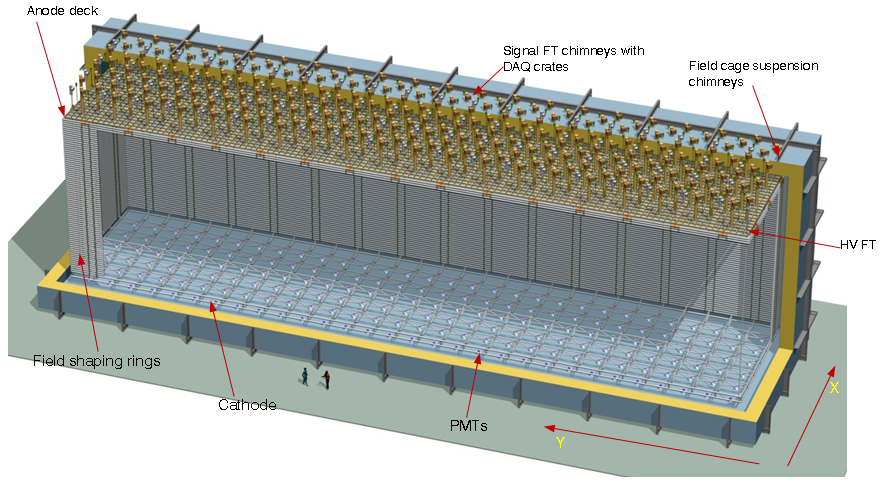
\includegraphics[width=\linewidth]{DUNE12_open}
\end{cdrfigure}

The field cage is held in place by mechanical structures hung from the
top deck of the vessel that also provide insulation.  The cathode
structure, constructed of a reinforced frame, to 
guarantee its planarity, is suspended from the field cage and hangs near the 
bottom of the cryostat. It is a segmented structure of tubes of different sizes 
arranged in a grid to minimize weight, limit sagging and avoid high electric field
regions in its proximity.  The segmented structure allows scintillation light to pass
through and be detected by uniform arrays of photomultipliers (PMTs) mounted
1~m below it at the bottom of the tank.

\section{Detector Configuration}

The detector for the \ktadj{12.1} active mass module is built as a single
active volume 60~m long, 12~m wide and 12~m high, with the anode at the
top, the cathode near the bottom and photon detectors underneath the cathode. 

The proposed design optimally exploits the
cryostat volume (14(w)$\times$14.1(h)$\times$62(l)~m$^3$) with an
anode active area of (12$\times$60~m$^2$) and a drift length of 12~m,
corresponding to an active mass of 12.096~kt of LAr (10.643~kt
fiducial).

 The design is based on the \ktadj{20} LAGUNA-LBNO design study
with a CRP unit size adapted to the dimensions on the active area. The
cryostat height could be increased to achieve 15-m drift, resulting in
an active mass of 15.12~kt (13.444~kt fiducial).  This \ktadj{15.1}
configuration, apart from the longer drift distance and field cage,
would have the same characteristics of the \ktadj{12.1} configuration,
given that the covered active area is exactly the same. With these
transverse dimensions, every additional meter of drift length provides
a \ktadj{1} increase in the active mass at a moderate additional cost.

The active volume (see Figure~\ref{fig:DP_det1} ) is surrounded by the
vertical field cage made of rectangular tubular rings 
\begin{cdrfigure}[Dual-phase detector 3D view]{DP_det1}{The DUNE dual-phase 
detector with cathode, PMTs, field cage and anode plane with chimneys.}
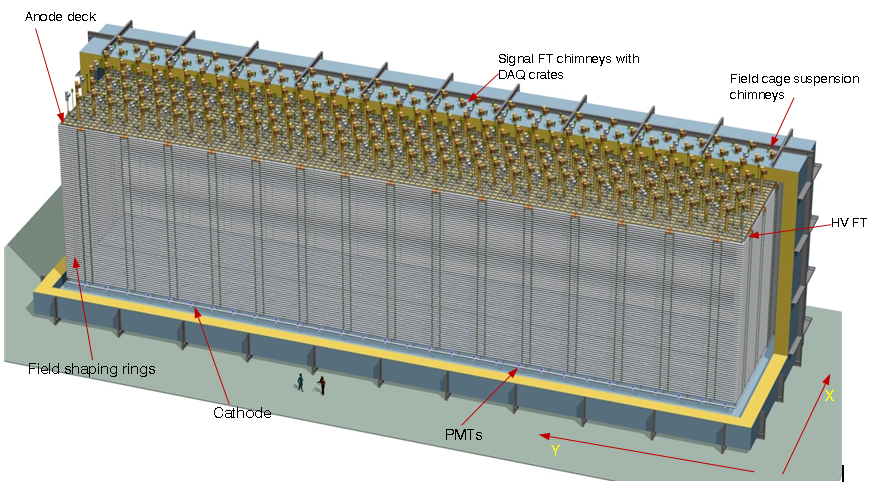
\includegraphics[width=\linewidth]{DUNE12_FC}
\end{cdrfigure}
The cathode plane (on the bottom) made by a reinforced frame filled by a tubular grid (not visible in
Figure~\ref{fig:DP_det2}) allows optical transparency for the scintillation light towards an array of 180 PMTs (1 per 4~m$^2$)
located at the bottom of the vessel.

The ionization electrons in the liquid phase drift  in a uniform electric field towards the anode plane at the top of the active
volume. This is made by by an array of 80 independent CRP modules, 3$\times$3~m$^2$ each.
The extraction of the electrons from the liquid to vapor phase is performed thanks to the submersed horizontal extraction grid, 
integrated in each CRP structure. A CRP unit includes 36 (0.5~m$\times$0.5~m) LEM/anode sandwiches, providing tunable
amplification and charge collection on two independent views organized in strips of 3~m length and 3.125~mm pitch. There are
1920 readout channels for each CRP. Signals in each CRP unit are collected via 3 signal feedthrough chimneys hosting the
the front-end cards with the cryogenic ASIC amplifiers (640 channels/chimney) which are accessible and replaceable without
contaminating the pure liquid argon volume. Each chimney is coupled to a microTCA crate ensuring the signals digitization and 
data acquisition. These crates are connected  via optical fiber links to the DAQ back-end. The total number of readout channel 
per 10 kt module is 153600.
 
Each CRP unit is independently suspended by 3 stainless steel ropes. The vertical level of each CRP unit can then be automatically
adjusted with respect to the LAr level via 3 suspension feedthroughs, electrically operated from outside. A Slow Control feedthrough, 
one per CRP unit, is used for the signals readout for level meters and the temperature probes and to apply the HV bias on the two
sides of the LEMs and on the extraction grid. The number of components and parameters for the \ktadj{12} (\ktadj{15})
dual-phase LArTPC are summarized in Tables~\ref{tab:DP_params}
and~\ref{tab:DP_numbers}.

\begin{cdrtable}[Sizes and Dimensions for the \ktadj{12} (\ktadj{15}) dual-phase LArTPC]{lll}
{DP_params}{Sizes and Dimensions for the \ktadj{12} (\ktadj{15}) dual-phase  LArTPC}  Item & Value(s) &  \\ \toprowrule
Active volume width and length & W = 12~m &  L = 60~m \\ \colhline
Active volume height &  H = 12~m (H = 15~m)  &  \\ \colhline
Active volume/LAr mass & 8,640 (10,800)~m$^3$ &  12,096 (15,120) metric ton \\ \colhline
Field ring vertical spacing & 200~mm  \\ \colhline
Field ring tube diameter & 140~mm \\ \colhline
Anode plane size & W = 12~m & L = 60~m \\ \colhline
CRP unit size & W = 3~m & L = 3~m  \\ \colhline
HV for vertical drift & 600--900~kV \\ \colhline
Resistor value & 100~M$\Omega$ \\ 
\end{cdrtable}
\begin{cdrtable}[Quantities of Items for the \ktadj{12} (\ktadj{15}) dual-phase LArTPC]{ll}{DP_numbers}{Quantities of Items for the \ktadj{12} (\ktadj{15}) dual-phase  LArTPC}  Item & Number    \\ \toprowrule
Field rings & 60  (75)  \\ \colhline
CRP units & 4 $\times$ 20 = 80 \\ \colhline
LEM/Anode sadwiches per CRP unit & 36 \\ \colhline
LEM/Anode sandwiches (total) & 2,880 \\ \colhline
SFT chimneys / CRP unit & 3 \\ \colhline
SFT chimneys (total) & 240 \\ \colhline
Readout channels / SFT chimney & 640  \\ \colhline
Readout channels (total) & 153,600 \\ \colhline
Suspension FT / CRP unit & 3  \\ \colhline
Suspension FTs (total) & 240  \\ \colhline
Slow Control FT / sub-anode & 1  \\ \colhline
Slow Control FTs (total) & 80 \\ \colhline
HV feedthrough & 1  \\ \colhline
Voltage degrader resistive chains & 4 \\ \colhline
Resistors (total) & 240 (300)  \\ \colhline
PMTs (total) & 180 (1/4~m$^2$) \\ 
\end{cdrtable}


A number of factors make the dual-phase TPC concept as described in this chapter 
well suited to large detector sizes like the DUNE Far Detector.

In this design, the charge attenuation on the long drift paths is compensated by the
charge amplification in the CRPs.  This configuration also simplifies
construction by optimally exploiting the long vertical dimensions of
the cryostat, providing a large homogeneous fiducial volume 
free of embedded passive materials (effectively increasing the detector size),
reducing the number of readout channels,  and ultimately lowering costs.  
The CRPs collect the charge in a projective way,  with practically no dead region and read the signals out 
in two collection views, eliminating the need for  induction views, which 
simplifies the reconstruction of complicated topologies. The tunable high S/N provides operative margins
with respect to the noise and electron lifetime conditions and lowers the threshold on the minimal
detectable energy depositions .

The dual-phase readout scheme has been successfully demonstrated on
several prototypes through R\&D over a span of more than 10 years.  The
design of very large (20--50~kt) underground detectors based on this
concept has been developed in great detail in the context of the
LAGUNA and LAGUNA-LBNO design studies.  The CERN WA105 demonstrator, 
described in Section~\ref{sec:proto-cern-double}, is intended to prototype 
a full-scale implementation of this technique, as
well as demonstrate other technologies developed for the construction of large
underground TPC detectors.  

 A complete configuration, based on the double-phase design, been optimized for the 10 kton
detector module of the DUNE Far Detector.